\documentclass[11pt,fleqn]{article}
\renewcommand{\baselinestretch}{1.3}
\usepackage[usenames,dvipsnames]{color}
\usepackage{hyperref,harvard,amsmath,amssymb,lscape,graphicx,setspace,cancel,amsthm,upquote}
%\usepackage{amsfonts,latexsym,eurosym}
\bibliographystyle{aer}

\pdfpagewidth 8.5in
\pdfpageheight 11in
\topmargin 0in
\headheight 0in
\headsep 0in
\textheight 9in
\textwidth 6.5in
\oddsidemargin 0in
\evensidemargin 0in
\headheight 0in
\headsep 0in

\newcommand{\D}{\displaystyle}
\newcommand{\E}{\begin{eqnarray*}}
\newcommand{\F}{\end{eqnarray*}}
\newcommand{\EE}{\begin{eqnarray}}
\newcommand{\FF}{\end{eqnarray}}
\newcommand{\IZ}{\begin{itemize}}
\newcommand{\ZI}{\end{itemize}}
\newcommand{\EN}{\begin{enumerate}}
\newcommand{\NE}{\end{enumerate}}
\newcommand{\itemc}{\item[$\circ$]}
\newcommand{\itemb}{\item[]}
\newcommand{\IZdash}{\begin{itemize} \renewcommand{\labelitemi}{-}}

\newcommand{\ttt}{\texttt}
\newcommand{\tn}{\textnormal}
\newcommand{\tc}{\textcolor}

\hypersetup{colorlinks=true,urlcolor=blue,linkcolor=black}

\singlespacing

%%%%%%%%%%%%%%%%%%%%%%%%%%%%%%%%%%%%%%%%%%%%%%%%%%%%%%%%%%%%%%%%%%%%%%%%%%%%%%%%%%%%%%%%%%%%%%%%%%%%
%%%%%%%%%%%%%%%%%%%%%%%%%%%%%%%%%%%%%%%%%%%%%%%%%%%%%%%%%%%%%%%%%%%%%%%%%%%%%%%%%%%%%%%%%%%%%%%%%%%%%

\begin{document}

\begin{titlepage}
\title{Documentation for the \ttt{fredpy} Python package}
\author{Brian C. Jenkins\thanks{Email: \href{mailto:bcjenkin@uci.edu}{bcjenkin@uci.edu} This project is ongoing and I welcome all feedback. I have no affiliation with the Federal Reserve Bank of St.~Louis or with any other component of the Federal Reserve System.}\\Department of Economics \\University of California, Irvine}
\date{\today}

\maketitle

\begin{abstract}
\noindent \ttt{fredpy} is a Python package for retrieving and working with data from Federal Reserve Economic Data (FRED). The package makes it easy to download specific data series and provides a set of tools for transforming the data in order to construct plots and perform statistical analysis. The \ttt{fredpy} package is useful for anyone doing empirical research using the data from FRED and for anyone, e.g.~economics teachers, students, and journalists, that will benefit from having an efficient and flexible way to access FRED with Python. \ttt{fredpy} is compatible with Python 2.7 and 3.4.
\end{abstract}

\thispagestyle{empty}
\end{titlepage}

\tableofcontents

\newpage
%%%%%%%%%%%%%%%%%%%%%%%%%%%%%%%%%%%%%%%%%%%%%%%%%%%%%%%%%%%%%%%%%%%%
%%%%%%%%%%%%%%%%%%%%%%%%%%%%%%%%%%%%%%%%%%%%%%%%%%%%%%%%%%%%%%%%%%%%

\section{Introduction}

Federal Reserve Economic Data or FRED is a rich database maintained but the Federal Reserve Bank of St.~Louis.\footnote{Site: \href{http://research.stlouisfed.org/fred2/}{http://research.stlouisfed.org/fred2/}} \verb=fredpy= is a Python package that simplifies the process of downloading and manipulating data from FRED. The package offers a streamlined way of retrieving data directly from the FRED website and provides a number of tools to assist with management of the series obtained. This package is particularly useful for creating Python programs that integrate data retrieval with statistical analysis. The package is also well-suited for use with programs that will update figures and tables as new data are released.


\section{Preliminaries}

Install the \ttt{fredpy} package by running \ttt{pip install fredpy} in the shell or by obtaining the tarball from \href{https://pypi.python.org/pypi/fredpy/0.1.0a}{PyPI}. \ttt{fredpy} has the following package dependencies:

\

\begin{tabular}{rl} 
 $\cdot$ & \ttt{matplotlib}\\
 $\cdot$ & \ttt{numpy}     \\
 $\cdot$ & \ttt{scipy}     \\ 
 $\cdot$ & \ttt{statsmodels}
\end{tabular}

\subsection{Initialization}

To create a \ttt{fredpy.series} instance, you must have the unique Series ID for the data that you wish to retrieve. Generally, you will find this by searching the FRED website for the data series by name. For example, use the FRED site to find that GDPC96 is the Series ID for real GDP of the US (quarterly frequency, seasonally adjusted). Create a \ttt{fredpy.series} instance based on this data:

\

\begin{minipage}{6.5in}
\ttt{>>>\tc{ForestGreen}{from} \tc{RoyalBlue}{fredpy} \tc{ForestGreen}{import} \tc{RoyalBlue}{series}}

\verb!>>>gdp = series('GDPC96')!
\end{minipage}

\

\noindent Now the \ttt{series} instance \ttt{gdp} is available for manipulation. 

Each \ttt{fredpy.series} instance is initialized with a set of attributes that describe the characteristics of the series retrieved from FRED. These attributes are:
	\IZ
	\itemb \ttt{title}: Title of the data.
	\itemb \ttt{source}: Original source of the data.
	\itemb \ttt{season}: Indicates whether the data has been seasonally adjusted.
	\itemb \ttt{freq}: Equals 365, 52, 12, 4, or 1 to indicate daily, monthly, quarterly, or annual frequency.
	\itemb \ttt{units}: Units of the data.
	\itemb \ttt{daterange}: Date range of data.
	\itemb \ttt{updated}: Date on which data was last updated.
	\itemb \ttt{idCode}: The unique FRED identification code for the series.
	\itemb \ttt{data}: A list containing the data.
	\itemb \ttt{dates}: A list containing date strings in yyy-mm-dd format.
	\itemb \ttt{datetimes}: A list containing the dates in \ttt{datetime} format for use with the \verb!plot_date! function from \ttt{matplotlib}.
	\ZI
In terms of the GDP example, find the precise title of data series used by FRED:

\

\begin{minipage}{6.5in}
\verb!>>> gdp.title!

\verb!'Real Gross Domestic Product, 3 Decimal'!
\end{minipage}

\

\noindent Or learn that the original source for the data series was the BEA:

\

\begin{minipage}{6.5in}
\verb!>>> gdp.source!

\verb!'U.S. Department of Commerce: Bureau of Economic Analysis'!
\end{minipage}

\

\noindent Or find out that quarterly real GDP data goes back to January 1947 and that, as of the time this document was written, the most recent observation was for the quarter beginning April 2014:

\

\begin{minipage}{6.5in}
\verb!>>> gdp.daterange!

\verb!'Range: 1947-01-01 to 2014-04-01'!
\end{minipage}

\

\noindent Several of the methods described in the next section will alter the values of the attributes created upon initialization. Furthermore, some methods -- the filtering methods in particular -- add a couple of new attributes as necessary.

\subsection{Methods}

Each \ttt{fredpy.series} instance has the following methods:

	\IZ	
	\itemb \ttt{pc(log=True)}
		\IZ
		\itemb Replaces the \ttt{data} attribute with the percentage change of the data series from the pervious time period. If \ttt{log=True}, then percentage changeis computed as the difference between the log of the current value and the log of the one period lag value:
			\EE
			100 \times \left[\log(X_t) - \log(X_{t-1})\right].
			\FF
		If \ttt{log=False}, then the percentage change is computed in the standard way:
			\EE
			100 \times \left[(X_t - X_{t-1})/X_{t-1}\right].
			\FF
		Also, method drops the first elements of the \ttt{dates} and \ttt{datetimes} attributes to account for the shorter observation window. Other attributes modified: \ttt{units} and \ttt{title}.
		\ZI
		
	\itemb \ttt{apc(log=True)}
		\IZ
		\itemb Replaces the \ttt{data} attribute with the \emph{annual} percentage change of the data series from the pervious time period. If \ttt{log=True}, then percentage change is computed as the difference between the log of the current value and the log of the one period lag value:
			\EE
			100 \times \left[\log(X_t) - \log(X_{t-k})\right],
			\FF
		where $k=1,4,12$, or $365$ is the annual frequency of the data series. If \ttt{log=False}, then the percentage change is computed in the standard way:
			\EE
			100 \times \left[(X_t - X_{t-k})/X_{t-k}\right].
			\FF
		Also, method drops the first $k$ elements of the \ttt{dates} and \ttt{datetimes} attributes to account for the shorter observation window. Other attributes modified: \ttt{units} and \ttt{title}.
		\ZI
	
	\itemb \ttt{ma2side(length)}
		\IZ
		\itemb Constructs a two-sided moving average with window of size $2\times\ttt{length}+1$. \emph{Note the different treatment of} \ttt{length} \emph{relative to the} \ttt{ma1side} \emph{method}. Adds attributes \ttt{ma2data}, \ttt{ma2dates}, \ttt{ma2datetimes}, and \ttt{ma2daterange}.
		\ZI
		
	\itemb \ttt{ma1side(length)}
		\IZ
		\itemb Constructs a one-sided (left side) moving average with window of size \ttt{length}. \emph{Note the different treatment of} \ttt{length} \emph{relative to the} \ttt{ma2side} \emph{method}. Adds attributes \ttt{ma1data}, \ttt{ma1dates}, \ttt{ma1datetimes}, and \ttt{ma1daterange}.
		\ZI
		
	\itemb \ttt{recent(N=10)}
		\IZ
		\itemb Constrains data series to the most recent \ttt{N} observations. The \ttt{dates} and \ttt{datetimes} attributes are adjusted from both ends to account for the reduced observation window. Other attributes modified: \ttt{daterange}
		\ZI
		
	\itemb \ttt{window(win)}
		\IZ
		\itemb Constrains data series to a specified window. \ttt{win} is a list specifying the minimum and maximum dates to be included. Dates must be in either mm-dd-yyyy or yyyy-mm-dd format. For example, to restrict observations to those between January 1, 1980 to December 31, 1999:
			\EE
			\verb!win=['01-01-1980','12-31-1999']!.
			\FF
		Other attributes modified: \ttt{daterange}
		\ZI
		
	\itemb \ttt{log()}
		\IZ
		\itemb Replaces the \ttt{data} attribute with the log of the data series. Other attributes modified: \ttt{title}
		\ZI
		
	\itemb \ttt{bpfilter(low=6,high=32,K=12)}
		\IZ
		\itemb Computes the bandpass (Baxter-King) filter of the series using the \ttt{statsmodels} package. Instead of replacing the modifying the original attributes, this method creates three new attributes:
			\IZ
            \itemb \ttt{bpcycle}: cyclical component of series
            \itemb \ttt{bpdates}: dates corresponding to bp filtered data
            \itemb \ttt{bpdatetimes}: date numbers corresponding to bp filtered data
            \ZI
       Method displays a warning if default values are used for \ttt{low}, \ttt{high}, and $\ttt{K}$ and the original series is not quarterly.
		\ZI
	
	\itemb \ttt{hpfilter(lamb=1600)}
		\IZ
		\itemb Computes the Hodrick-Prescott filter of the series using the \ttt{statsmodels} package. Instead of replacing the modifying the original \ttt{data} attribute, this method creates two new attributes:
			\IZ
            \itemb \ttt{hpcycle}: cyclical component of series
            \itemb \ttt{hptrend}: trend component of series
            \ZI
		Method displays a warning if default value is used for \ttt{lamb} and the original series is not quarterly.
        \ZI
		
	\itemb \ttt{cffilter(low=6,high=32,drift=True)}
		\IZ
		\itemb Computes the Christiano-Fitzgerald filter of the series using the \ttt{statsmodels} package. Instead of replacing the modifying the original \ttt{data} attribute, this method creates two new attributes:
			\IZ
            \itemb \ttt{cfcycle}: cyclical component of series
            \itemb \ttt{cftrend}: trend component of series
            \ZI
		Method displays a warning if default values are used for \ttt{low}, \ttt{high}, and $\ttt{drift}$ and the original series is not quarterly.
        \ZI
	
	\itemb \ttt{lintrend()}
		\IZ
		\itemb Computes the linear trend of the series. Instead of replacing the modifying the original \ttt{data} attribute, this method creates two new attributes:
			\IZ
            \itemb \ttt{lincycle}: cyclical component of series
            \itemb \ttt{lintrend}: trend component of series
            \ZI
		Method displays a warning if the original series is not quarterly.
        \ZI
		
	\itemb \ttt{firstdiff()}
		\IZ
		\itemb Computes the first-difference of the series. Instead of replacing the modifying the original \ttt{data} attribute, this method creates four new attributes:
			\IZ
            \itemb \ttt{diffcycle}: cyclical component of series
            \itemb \ttt{difftrend}: trend component of series
            \itemb \ttt{diffdates}: shorter date sequence
            \itemb \ttt{diffdatetimes}: shorter date numbers
            \itemb \ttt{diffdata}: shorter data series
            \ZI
        \ZI
		
	\itemb \verb!monthtoquarter(method='average')!
		\IZ
		\itemb Converts series with monthly frequency to quarterly frequency. Modifies \ttt{data}, \ttt{dates}, \ttt{datetimes}, \ttt{t} attributes. If \verb!method='average'!, then the value for a quarter is the average over each month of the corresponding three month period. If \verb!method='sum'!, then the value for a quarter is the sum over the months of the corresponding three month period. And if \verb!method='end'!, then the value for a quarter is value of the last  month of the corresponding three month period. 
		\ZI		
	
	\newpage	
	\itemb \verb!quartertoannual(method='average')!
		\IZ
		\itemb Converts series with quarterly frequency to annual frequency. Modifies \ttt{data}, \ttt{dates}, \ttt{datetimes}, \ttt{t} attributes. If \verb!method='average'!, then the value for a year is the average over each quarter of the corresponding four quarter period. If \verb!method='sum'!, then the value for a year is the sum over the quarters of the corresponding four quarter period. And if \verb!method='end'!, then the value for a year is value of the last  quarter of the corresponding four quarter period. 
		\ZI		
	
	\itemb \verb!monthtoannual(method='average')!
		\IZ
		\itemb Converts series with monthly frequency to annual frequency. Modifies \ttt{data}, \ttt{dates}, \ttt{datetimes}, \ttt{t} attributes. If \verb!method='average'!, then the value for a year is the average over each month of the corresponding twelve month period. If \verb!method='sum'!, then the value for a year is the sum over the months of the corresponding twelve month period. And if \verb!method='end'!, then the value for a year is value of the last  month of the corresponding twelve month period.  
		\ZI				
		
		
	\itemb \verb!percapita(total_pop=True)!
		\IZ
		\itemb Replaces the \ttt{data} attribute with the values divided by the US population using one of two definitions of population:
			\IZ
            \itemb \verb!total_pop=True!: total population US population.
            \itemb \verb!total_pop=False!: civilian noninstitutional population is defined as persons 16 years of age and older.
			\ZI
		Other attributes modified: \ttt{title} and \ttt{units}
		\ZI		
		
	\itemb \ttt{recessions()}
		\IZ
		\itemb Creates gray recession bars for plots. Should be used after a plot has been made but
            before either (1) a new plot is created or (2) a show command is issued.
		\ZI
	\ZI
	
\subsection{Other Functions}

The \verb!fredpy! package is equipped with two functions that are occasionally useful for working with \ttt{fredpy.series} objects:

	\IZ
	\itemb \verb!quickplot(x,year_mult=10,show=True,recess=False,save=False,name='file',width=2)!
		\IZ
		\itemb This function produces a plot of the data for a given \ttt{fred} instance \ttt{x}. \verb!year_mult! specifies the multiple in which years on the horizontal axis should be formed. \verb!show=True! means that a new plot window should be created. \verb!recess=False! means that no recession bars should be plotted and \verb!recess=True! means the opposite. If \verb!save=True!, the plot is saved in .png format. \ttt{width} specifies the width of the plotted line.
		\ZI
		
	\itemb \verb!window_equalize(series_list)!
		\IZ
		\itemb Equalizes the data windows for a list of \ttt{fredpy.series} instances by finding the largest date range for which there is data available from each series in \verb!series_list!. 
		\ZI
	\ZI
	
\section{Examples}

\subsection{Example 1: Plotting with the \ttt{quickplot} function}


To begin, let's construct a plot of all currently available data for the US unemployment rate. To do this, we run a script that contains the following:

\

\begin{minipage}{6.5in}
\ttt{\tc{ForestGreen}{from} \tc{RoyalBlue}{fredpy} \tc{ForestGreen}{import} \tc{RoyalBlue}{series, quickplot}}

\verb!unemp = series('UNRATE')!

\verb!quickplot(unemp,recess=True,save=True,name='fredpy_example1')!

\

\end{minipage}

\noindent This program will display a plot and will save the plot to a file called \verb!fredpy_example1.png! in the working directory. The output is depicted in figure \ref{fig:1}. The quick plot function has the advantage of being able to generate plots on the fly, but most of the time you will want to mange plotting directly.

\begin{figure}[h] \caption{\label{fig:1} A plot of the US unemployment rate using the \ttt{quickplot} function.}
\begin{center}
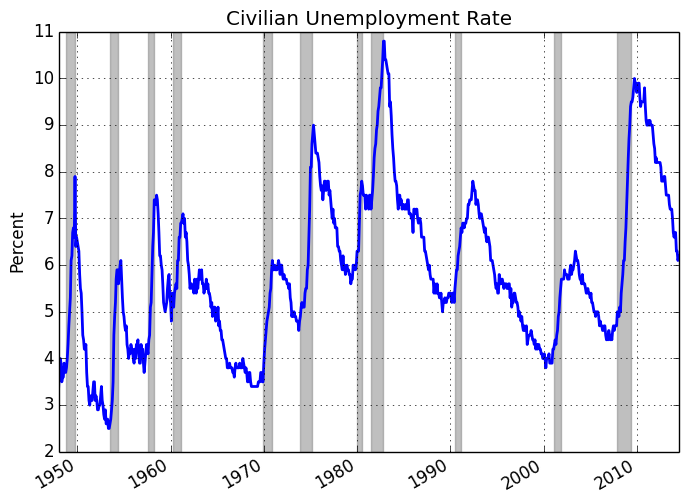
\includegraphics[height = 10cm]{fig_fredpy_example1.png}
\end{center}
\end{figure}

\subsection{Example 2: Plotting Multiple Series}

Next we will construct a more elaborate plot using the \ttt{fredpy}. The objective is to create a four-panel plot containing the rate of real GDP growth, CPI inflation, the unemployment rate, and the 3-month T-bill rate. Since the available ranges for these series are different, we will make use of the \verb!window_equalize! function to make sure that we plot all four series over the same date range. First, the import statements:

\

\begin{minipage}{6.5in}
\ttt{\tc{ForestGreen}{import} \tc{RoyalBlue}{matplotlib.pyplot} \tc{ForestGreen}{as} \tc{RoyalBlue}{plt}}

\ttt{\tc{ForestGreen}{from} \tc{RoyalBlue}{fredpy} \tc{ForestGreen}{import} \tc{RoyalBlue}{series, window\_equalize}}

\ttt{\tc{ForestGreen}{import} \tc{RoyalBlue}{matplotlib.dates} \tc{ForestGreen}{as} \tc{RoyalBlue}{dts}}

\ttt{\tc{ForestGreen}{from} \tc{RoyalBlue}{datetime} \tc{ForestGreen}{import} \tc{RoyalBlue}{dates}}

\

\end{minipage}

\noindent Next, download data from FRED:

\

\begin{minipage}{6.5in}
\verb!gdp = series('GDPC96')!

\verb!cpi = series('CPIAUCSL')!

\verb!unemp=series('UNRATE')!

\verb!tbill=series('TB3MS')!

\

\end{minipage}

\noindent Then replace divide gdp data by 1{,}000 to convert units from billions of dollars to trillions of dollars.

\

\begin{minipage}{6.5in}

\ttt{gdp.data = gdp.data/1000}

\

\end{minipage}

\noindent Use the \ttt{apc()} method to compute annual growth in real GDP and the CPI. Note that this method computes percentage change \emph{from one year previous}.

\

\begin{minipage}{6.5in}
\ttt{gdp.apc()}

\ttt{cpi.apc()}

\

\end{minipage}

\noindent Now use the \ttt{window\_equalize} function to set the date ranges to the smallest range common to all four series.

\

\begin{minipage}{6.5in}
\verb!series_list = [gdp,cpi,unemp,tbill]!

\verb!window_equalize(series_list)!

\

\end{minipage}

\noindent Finally, plot the data. Take note of the plot syntax. Use the function \verb!plot_date()! to plot the data of each \ttt{fred}object against its date numbers.

\

\begin{minipage}{6.5in}
\ttt{fig = plt.figure()}

\ttt{years10  = dts.YearLocator(10)}

\
\end{minipage}


\begin{minipage}{6.5in}
\ttt{\tc{Magenta}{\# plot real gdp growth}}

\verb!ax1 = fig.add_subplot(221)!

\verb!ax1.plot_date(gdp.datetimes,gdp.data,'b-',lw = 3)!

\verb!ax1.xaxis.set_major_locator(years10)}!

\verb!ax1.yaxis.set_major_formatter(y_format)!

\verb!ax1.set_ylabel('Trillions of 2009 $')!

\verb!fig.autofmt_xdate()!

\ttt{ax1.grid(True)}

\ttt{gdp.recessions()}

\verb!ax1.set_title('Real GDP')!

\

\end{minipage}

\begin{minipage}{6.5in}
\ttt{\tc{Magenta}{\# plot cpi inflation}}

\verb!ax2 = fig.add_subplot(222)!

\verb!ax2.plot_date(cpi.datetimes,cpi.data,'b-',lw = 3)!

\verb!ax2.xaxis.set_major_locator(years10)!

\verb!ax2.set_ylabel('Percent')!

\verb!fig.autofmt_xdate()!

\ttt{ax2.grid(True)}

\ttt{cpi.recessions()}

\verb!ax2.set_title('CPI Inflation')!

\

\end{minipage}

\begin{minipage}{6.5in}
\ttt{\tc{Magenta}{\# plot unemployment rate}}

\verb!ax3 = fig.add_subplot(223)!

\verb!ax3.plot_date(unemp.datetimes,unemp.data,'b-',lw = 3)!

\verb!ax3.xaxis.set_major_locator(years10)!

\verb!ax3.set_ylabel('Percent')!

\verb!fig.autofmt_xdate()! 

\ttt{ax3.grid(True)}

\ttt{unemp.recessions()}

\verb!ax3.set_title('Unemployment Rate')!

\

\end{minipage}

\begin{minipage}{6.5in}
\ttt{\tc{Magenta}{\# plot 3-mo T-bill rate}}

\verb!ax4 = fig.add_subplot(224)!

\verb!ax4.plot_date(tbill.datetimes,tbill.data,'b-',lw = 3)!

\verb!ax4.xaxis.set_major_locator(years10)!

\verb!ax4.set_ylabel('Percent')!

\verb!fig.autofmt_xdate()!

\ttt{ax4.grid(True)}

\ttt{tbill.recessions()}

\verb!ax4.set_title('3-mo T-bill Rate')!

\

\verb!plt.savefig('fredpy_example2.png',bbox_inches='tight')!

\ttt{plt.show()}

\

\end{minipage}

\noindent Figure \ref{fig:2} contains the output of this program.

\begin{figure}[h] \caption{\label{fig:2} Plots of real GDP growth, CPI inflation, the unemployment rate and the 3-moth T-bill rate.}
\begin{center}
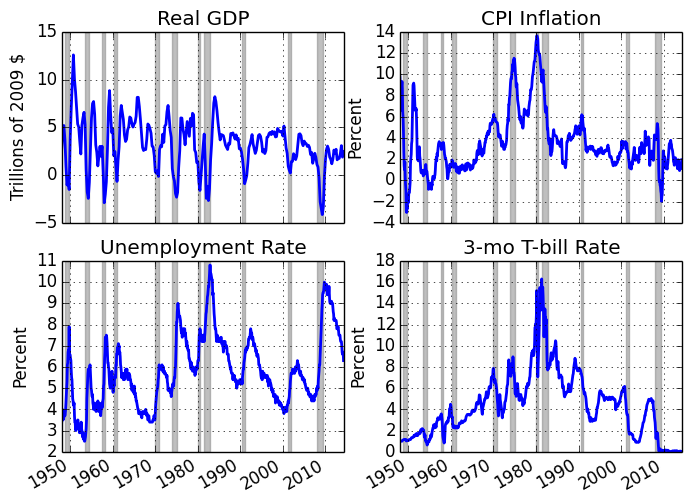
\includegraphics[height = 10cm]{fig_fredpy_example2.png}
\end{center}
\end{figure}


\subsection{Example 3: Filtering}

In the final example, we will use the Hodrick-Prescott (HP) and the Bandpass (BP) filters to isolate the business cycle components of real US GDP. Specifically, we will filter log per capita real GDP so that the resulting series may be interpreted as the log-deviations from trend.

\

\begin{minipage}{6.5in}
\ttt{\tc{ForestGreen}{import} \tc{RoyalBlue}{matplotlib.pyplot} \tc{ForestGreen}{as} \tc{RoyalBlue}{plt}}

\ttt{\tc{ForestGreen}{from} \tc{RoyalBlue}{fredpy} \tc{ForestGreen}{import} \tc{RoyalBlue}{series, window\_equalize}}

\ttt{\tc{ForestGreen}{import} \tc{RoyalBlue}{matplotlib.dates} \tc{ForestGreen}{as} \tc{RoyalBlue}{dts}}

\

\end{minipage}

\noindent Then download real GDP data from FRED and convert into units of log thousands of dollars per person.

\

\begin{minipage}{6.5in}
\verb!gdp = fred('GDPC96')!

\ttt{gdp.percapita()}

\ttt{gdp.data = gdp.data/1000}

\ttt{gdp.log()}

\

\end{minipage}

\noindent Apply the filters. The filter defaults are set for quarterly data.

\

\begin{minipage}{6in}
\ttt{gdp.bpfilter()}

\ttt{gdp.hpfilter()}

\

\end{minipage}

\noindent Finally, plot the data.

\

\begin{minipage}{6in}
\ttt{fig = plt.figure()}

\ttt{years10  = dts.YearLocator(10)}

\

\verb!ax1 = fig.add_subplot(111)!

\verb!ax1.plot_date(gdp.datetimes,gdp.hpcycle,'b-',lw = 2)!

\verb!ax1.plot_date(gdp.bpdatetimes,gdp.bpcycle,'r--',lw = 2)!

\verb!ax1.xaxis.set_major_locator(years10)!

\verb!ax1.set_ylabel('Percent')!

\verb!fig.autofmt_xdate()!

\ttt{ax1.grid(True)}

\ttt{gdp.recessions()}

\verb!ax1.legend(['HP','BP'],loc='lower right')!

\

\verb!plt.savefig('fredpy_example3.png',bbox_inches='tight')!

\ttt{plt.show()}

\

\end{minipage}

\noindent The output of the program is contained in Figure \ref{fig:3}.

\begin{figure}[h] \caption{\label{fig:3} HP and BP filtered log real GDP per capita.}
\begin{center}
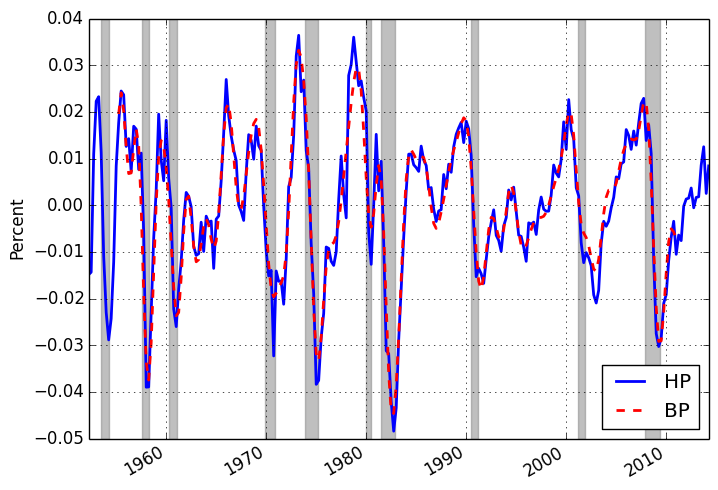
\includegraphics[height = 10cm]{fig_fredpy_example3.png}
\end{center}
\end{figure}


\section{Comments}

The examples above emphasize the ease with which the \ttt{fredpy} package is used for downloading data and making plots. For another example in this spirit, check out my \href{http://youtu.be/34bIQGrndao}{animation} of the US Treasury yield curve. Like all other \ttt{fredpy}-related materials, the code for this animation is also available from my \href{https://github.com/letsgoexploring/fredpy-package}{Github repository} or from my personal \href{http://www.briancjenkins.com/code/fredpy.html}{website}.

The \ttt{fredpy} package has uses beyond simple data visualization. A researcher doing statistical analysis using series available from FRED can use the package to create a single Python program -- or set of programs -- that retrieves data from FRED, performs the analysis, and exports to \LaTeX \ tables. Such functionality will reduce the researchers' time spent managing data files and will allow results to be upadted easily as new data become available.
\end{document}
